
\chapter{Finite Element Method}
\label{chap:Finite-Element-Method}

\section{Introduction} %#######################################################################

The determination of the solid-rotor induction motor performance has to be carried out through
the solution of Maxwell’s field equations. In order to take into account the whole machine
geometry, a large number of partial differential equations or integral equations have to be
solved. An effective and widely used method of numerically computing eddy-current fields is the
finite element analysis. For accurately solving distributed eddy-current problems containing
partial differential equations or integral equations an effective computer program is a useful
tool.

The comprehensive considerations and covering equations for the finite element method are
reported for instance by [30], [31] and [32]. The leading process in FEM is subdividing the
described machine geometry into portions for which a particular covering equation is valid. The
described geometrical portions are further subdivided into a large amount of smaller elements,
finite elements. The sizes of finite elements should be well proportioned in the motor geometry
and, especially, the meshing of the air gap should be done carefully. The air gap is divided
into three layers of equal width: the outer and inner layers are static and the middle layer is
the dynamic layer in which the meshing is regenerated for each time step. In saturating parts –
such as a solid rotor – the maximum element size is usually considered to be one third of the
depth of penetration. Although a fine meshing requires a long computation time, special
attention has to be paid also to the meshing of the rotor to accurately describe the complex
eddy-current problem in the ferromagnetic solid rotor.

Therefore, a very dense meshing of the rotor and, in particular, on its outer layers is
preferred.

\begin{figure}[t]
  \begin{center}
    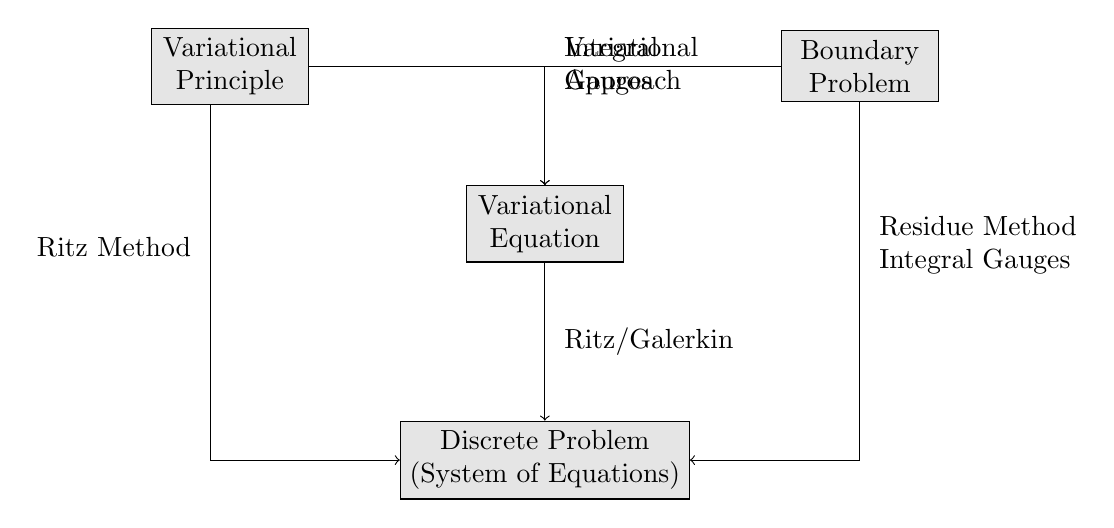
\begin{tikzpicture}[%
      block/.style={%
        minimum width = 2cm,
        fill          = gray!20,
        align         = center,
        draw          = black,
        node distance = 4cm,
        top color      = gray!20,
        bottom color   = gray!20!white,
      }
      ]

      \node[block] (Var-Prip) at (0,0) {Variational \\ Principle};
      \node[block] (BVP) at (8,0) {Boundary \\ Problem};
      \node[block] (Var-Eq) at (4,-2) {Variational \\ Equation};
      \node[block] (Sys-Eq) at (4,-5) {Discrete Problem \\ (System of Equations)};

      \draw[->] ([xshift=0.5cm]Var-Prip) -| node[label={[align=left]right:Variational \\ Approach}] {}  (Var-Eq);
       \draw[->] ([xshift=-0.5cm]BVP) -| node[label={[align=left]right:Integral \\ Gauges}] {}  (Var-Eq);

      \draw[->] (Var-Eq) -- node[label={right:Ritz/Galerkin}] {}  (Sys-Eq);
      \draw[->] ([xshift=-2.5cm]Var-Prip) |- node[pos=0.2,label={left:Ritz Method}] {} (Sys-Eq) ;
      \draw[->] (BVP) |- node[pos=0.2,label={[align=left]right:Residue Method \\ Integral Gauges}] {} (Sys-Eq) ;
      
    \end{tikzpicture}
  \end{center}
  \caption{A Flow chart for finite element method.}
\end{figure}

\section{Maxwell's Equations} %################################################################

The electromagnetic behavior exhibited during the normal operation of electrical machinery can
be explained using Maxwell’s Equations. Faraday’s indution law determines the connection
between the electric field strength E and the magnetic flux density B. Amperé’s law give that
the relation between magnetic field strenth H and current density J and the changing of the
electric flux density D.

\begin{align}
  \nabla\times E = - \frac{\partial B}{\partial t}
\end{align}

\section{Modelling Losses} %###################################################################


\subsection{Stator Core Losses} %~~~~~~~~~~~~~~~~~~~~~~~~~~~~~~~~~~~~~~~~~~~~~~~~~~~~~~~~~~~~~~

Time-changing magnetic fields in ferromagnetic materials are the main reason
for the magnetic iron losses happening in the motor. These losses include the
hysteresis losses Phys which caused by the magnetic hysteresis loop of the
ferromagnetic material and eddy current losses. These eddy current losses are
separated into two types of losses which are as follows;
\begin{itemize}
\item Classical eddy current losses (Pclass)
 \item  Excess losses (Pabnormal) which is mainly caused by non-uniform distributions of
  magnetic flux density in the lamination. This occurs because of the grain properties
  of the ferromagnetic material [16]
\end{itemize}


The hysteresis losses which are caused by the AC magnetization process are
equal to the total area of the quasi-static hysteresis loop times the magnetizing
frequency in addition to the volume of the core [18]. The total loss energy per cycle
of the hysteresis loop can be seen in (3.4)

The hysteresis losses in a motor can be approximately calculated using
Steinmetz formula which is based on empirical studies.
%
\begin{equation}\label{eq:mag-loss-5}
  P_{hys} =
  k_{h} f B_{m}^{2}
\end{equation}
%
Where kh is the hysteresis constant which is related to the nature of the
material used, f is the frequency and Bm is the maximum magnetic flux density.
The eddy current losses that is occurred in the system is caused by the
induced electric currents in the magnetic core by an external time changing magnetic
field. These losses can be seen in (4.6)
%
% 4.6
%
The eddy current loss constant, keddy, is related to the conductivity and the
thickness of the material used [32]. Because of the difference of magnetic flux
density in the yoke and teeth of the stator core, it is logical to divide the losses into
two categories. Because of the way stators are constructed, some unwanted
construction defects occur which in turn causes the increase in eddy current losses. In
light of all this the total hysteresis and eddy current losses can be calculated using the
equations given below;
%
% 4.7-4.9
%
Where v10 is the total iron loss constant which is calculated in (4.9), Bteeth,1/3
and Byoke are the magnetic flux densities at the stator teeth at 1/3 of the tooth length
and the stator yoke respectively , mteeth and myoke are the total mass of the teeth and
the yoke respectively. bsh is the thickness of the selected loss stator laminated steel
and kf is the lamination staking factor.

For use in the study, the stator iron losses are calculated using numerical
methods using the Bertotti formula given in (4.10) [33]. So a non-sinusoidal time
variation of B(t) can be calculated, including the effect of abnormal losses. In (4.10)
it is considered, that B(t) is made up of a fundamental sinusoidal variation B(t) with
the frequency f and the deviation of that does not affect the hysteresis losses.
%
% 4.10
% 
Where p(t) is the specific iron loss per volume of the iron core, kf is the lamination
stacking factor, kh is the hysteresis loss constant, Bm is the maximum flux density of
the fundamental sinusoidal time variation, f is the operation frequency, κ is the
electrical conductivity of the core sheets, bsh is the lamination thickness and kex is the
abnormal eddy current losses constant.

\subsection{Rotor Eddy-Current Losses} %~~~~~~~~~~~~~~~~~~~~~~~~~~~~~~~~~~~~~~~~~~~~~~~~~~~~~~~

When the systems are modelled in FEM, the time variation of the stator
voltage and the current are given in pure sinusoidal forms. When the spatial
distribution of flux density that occurs in the air gap is concerned a pure sinusoidal
hypothesis would not work. The space distribution of the flux density has no
correlation to the time variation of the time current that is being fed to the windings.
This phenomena occurs only on the winding arrangement in the slots and on the
rotors own geometry.

The rotor eddy current losses Peddy is made up from the fundamental
component P., which dependent of the rotor frequency, and high frequency eddy
current losses Pftr,add . Which is caused by slotting [34]. These rotor eddy current
losses were numerically calculated with the aid of FEM simulation using (4.11) [20,
21].
%
% 4.11
%
In (4.11) the constant ρ represents the specific electrical resistance of the rotor steel.
The calculations were done with the aid of FEM.
The total amount of eddy current loss density that occurs in the rotor can be
categorized in three sections;

\begin{itemize}
\item High value eddy current loss beneath the rotor surface with a penetration  depth of d
  \item Eddy current loss that occurs in the teeth
\item   Eddy current loss that occurs in the yoke
\end{itemize}

In light of all this the total loss of eddy currents can be summed in (4.13)

\subsection{Joule (Electrical) Losses} %~~~~~~~~~~~~~~~~~~~~~~~~~~~~~~~~~~~~~~~~~~~~~~~~~~~~~~~

Electrical or Joule losses happens when the current passes through a
conductor and because of the conductors resistance gives of energy in term of heat.
These losses include the current with the fundamental and harmonic frequencies and
also include the losses that is caused by the current displacement. The total amount
of winding losses are the sum of I2R (ohmic) losses , the 1st order current
displacement losses Pcu,1 which happens because of the unbalanced current sharing
between the parallel wires per turn and finally the 2nd order displacement losses
which occurs because of the skin effect within each wire.

Rs, which is the phase resistance, is in direct relation with the operating temperature.
When the motor is in operation, the current I flows through the winding conductors.
These current that flow through the conductor, depending on the frequency and the
geometry, induce eddy currents mainly in the slot part of the conductors. Due to
these eddy currents, the total conductor current density J is displaced within the
conductor cross-section. This phenomena is also known as “skin effect”. In relation
to all aforementioned above, the second order current displacement causes the
increase on Stator AC resistance which in turn increase the Joule losses. In addition,
the first order current displacement losses happens because of the uneven distribution
on parallel wires per turn which can me measures given in [35][36];
%
\begin{equation}\label{eq:mag-14}
  R_{S} =
  R_{S,\,20}
  \left(1 + \frac{\theta - \theta_{0}}{235 + \theta_{0}}\right)
\end{equation}
%
In the equation given above, RS,20 is the phase winding dc-resistance at V0 = 20 and ϑ
is the winding operating temperature
%
% 4.15
%
While high speed motors can operate at higher frequencies than conventional motors,
the current displacement that is caused by the internal eddy currents are more
prominent at loss calculations. When a Dc current is applied it effect the conductor
evenly but, when an AC current is applied this is not the case (“Skin Effect”). The
current penetration depth is defined usually as the main boundary of the region, the
part where the most of the current flows. Since this area is only some part of the
conductors area, the resistance for the AC current is higher which also effects the
first and the second order current displacement. This increase in AC winding
resistance also directly affect the winding losses, which are calculated in (4.16) and
(4.22) [37]
%
% 4.16 - 4.22
%
